\section{Skellam-based Gaussian approximation}%???????
\label{app:bessel}
In this section, we present another way of approximating Eq.~\eqref{eq:accurate}, which we duplicate here for convenience:
\begin{equation}
  P=e^{-\eta_1|\alpha_1|^2}e^{-\eta_2|\alpha_2|^2}
\left(\frac{\eta_1|\alpha_1|^2}{\eta_2|\alpha_2|^2}\right)^{\frac{\delta m}{2}}
I_{\delta m}\left(2\sqrt{\eta_1\eta_2|\alpha_1|^2|\alpha_2|^2}\right),\label{eq:Skellam}
\end{equation}
%where $I_k(z)$ is the modified Bessel function of the first kind, and the transformed amplitudes $|\alpha_{1,2}|$ are given by Eq.~\eqref{eq:amplitudes}.


In the strong LO approximation, where $|\alpha_L|\gg|\alpha|$, the Bessel function $I_k(z)$ can be approximated using its asymptotic expression for large $|z|$ and $k$, with finite $\sqrt{\left|\frac{k^2}{z}\right|}$ (see Ref.~\cite{doi:10.1080/09500349808231235,freyberger1993photon}),
\begin{equation}
    I_k(z)\approx\frac{1}{\sqrt{2\pi z}}\exp\left[z-\frac{k^2}{z}\right]. \label{eq:hole}
\end{equation}
Assuming $C\not\to0$ and $S\not\to0$, (which avoids contradictions in the strong LO approximation as per Eq.~\eqref{eq:amplitudes}) and that $(CS)^{-1}$ remains finite, we can approximate the terms in the Skellam distribution as follows:
\begin{equation}
    |\alpha_1||\alpha_2|
    \approx
    CS|\alpha_L|^2\left[1+\frac{C^2-S^2}{(CS)^2}\frac{2CS\Re\alpha\alpha_L^*}{|\alpha_L|^2}\right]^{\frac{1}{2}}
    \approx
    CS|\alpha_L|^2+\left(C^2-S^2\right){\Re\alpha\alpha_L^*},
\end{equation}
\begin{multline}
    \exp\left[
    2\sqrt{\eta_1\eta_2}|\alpha_1||\alpha_2|-\eta_1|\alpha_1|^2-\eta_2|\alpha_2|^2
    \right]\approx
\\
    \approx\exp\left[-\left(|\alpha_L|(S\sqrt{\eta_1}-C\sqrt{\eta_2})+\frac{CS\Re\alpha\alpha_L^*}{|\alpha_L|}\left\{S\sqrt{\eta_1}+C\sqrt{\eta_2}\right\}\right)^2\right],
\end{multline}
\begin{equation}
        \left(\frac{{\eta_1}|\alpha_1|^2}{{\eta_2}|\alpha_2|^2}\right)^{\frac{\delta m}{2}}\approx
    \exp\left[\frac{\delta m}{2}\left(
    \ln\frac{\eta_1S^2}{\eta_2C^2}+\frac{2\Re\alpha\alpha_L^*}{CS|\alpha_L|^2}\right)
    \right],
    \label{eq:hole2}
\end{equation}
then we obtain the following approximation of Eq.~\eqref{eq:Skellam}:
\begin{multline}
        P_B=
    \frac{1}{\sqrt{4\pi\sqrt{\eta_1\eta_2}\left(CS|\alpha_L|^2+(C^2-S^2){\Re\alpha\alpha_L^*}\right)}}
    \times\\\times\exp\biggl[
    -\frac{\delta m^2}{4\sqrt{\eta_1\eta_2}\left(CS|\alpha_L|^2+\left(C^2-S^2\right){\Re\alpha\alpha_L^*}\right)}-\\-\left(
|\alpha_L|(S\sqrt{\eta_1}-C\sqrt{\eta_2})+\frac{CS\Re\alpha\alpha_L^*}{|\alpha_L|}\left\{
S\sqrt{\eta_1}+C\sqrt{\eta_2}
\right\}
\right)^2
    +\\+
    \frac{\delta m}{2}\left(
    \ln\frac{\eta_1S^2}{\eta_2C^2}+\frac{4CS\Re\alpha\alpha_L^*}{|\alpha_L|^2}\right)
    \biggr],
\end{multline}
which simplifies to:
\begin{multline}
    P_B=\frac{1}{\sqrt{4\pi\sqrt{\eta_1\eta_2}\left(CS|\alpha_L|^2+(C^2-S^2)\Re\alpha\alpha_L^*\right)}}
    \times\\\times\exp\biggl[-\frac{1}{2}\frac{\sqrt{\eta_1\eta_2}}{2CS}
    \biggl(\frac{\delta m}{{\sqrt{\eta_1\eta_2}|\alpha_L|}}-
    CS|\alpha_L|\ln\frac{\eta_1S^2}{\eta_2C^2}-\langle\hat{x}_\phi\rangle
    \biggr)^2\biggr],\label{eq:Pbad}
\end{multline}
to this we will refer as "Skellam-based Gaussian approximation".
Note that Eq.~\eqref{eq:Pgood} and Eq.~\eqref{eq:Pbad} are equivalent for the symmetric case. However, expressing $P_B$ in the form of Eq.~\eqref{eq:theform} and using Eq.~\eqref{eq:conv} gives
\begin{equation}
    2\frac{2CS}{\sqrt{\eta_1\eta_2}}=\sigma+2.
\end{equation}
This implies that $\sigma$ can be negative for certain combinations of $\eta_{1,2}$ and $\theta$ (e.g $\eta_1+\eta_2<2, \theta\neq{\pi}/{4}$), which contradicts the form given in Eq.~\eqref{eq:theform}. Therefore, Eq.~\eqref{eq:Pbad} does not fully describe the asymmetrical case, and this is a direct consequence of Eq.~\eqref{eq:hole}. Numerical results (see Fig.~\ref{fig:PB_PG}) also indicate that $P_B$ is less accurate than $P_G$ for approximating Eq.~\eqref{eq:accurate} in cases of higher asymmetry. Moreover, we can pinpoint the cause of worse performance to terms given by Eq.~\eqref{eq:hole} and Eq.~\eqref{eq:hole2}. We draw this conclusion from the difference in shifting of exact and approximate formulae, which are described by these terms. To further prove this, we will calculate the relation:
\begin{equation}
    \frac{I_{\delta m}(z)
    }{\frac{1}{\sqrt{2\pi z}}\exp\left[z-\frac{k^2}{z}\right]}
    \frac{\left(\frac{{\eta_1}|\alpha_1|^2}{{\eta_2}|\alpha_2|^2}\right)^{\frac{\delta m}{2}}}{\exp\left[\frac{\delta m}{2}\left(
    \ln\frac{\eta_1S^2}{\eta_2C^2}+\frac{2\Re\alpha\alpha_L^*}{CS|\alpha_L|^2}\right)
    \right]}
    ,\label{eq:relation}
\end{equation}
where $z\equiv2\sqrt{\eta_1\eta_2|\alpha_1|^2|\alpha_2|^2}$, as a function of $\theta$. Results are presented in Fig.~\ref{fig:relation}, from which we may see that at high asymmetry these approximations do not hold.
\begin{figure}
    \centering
    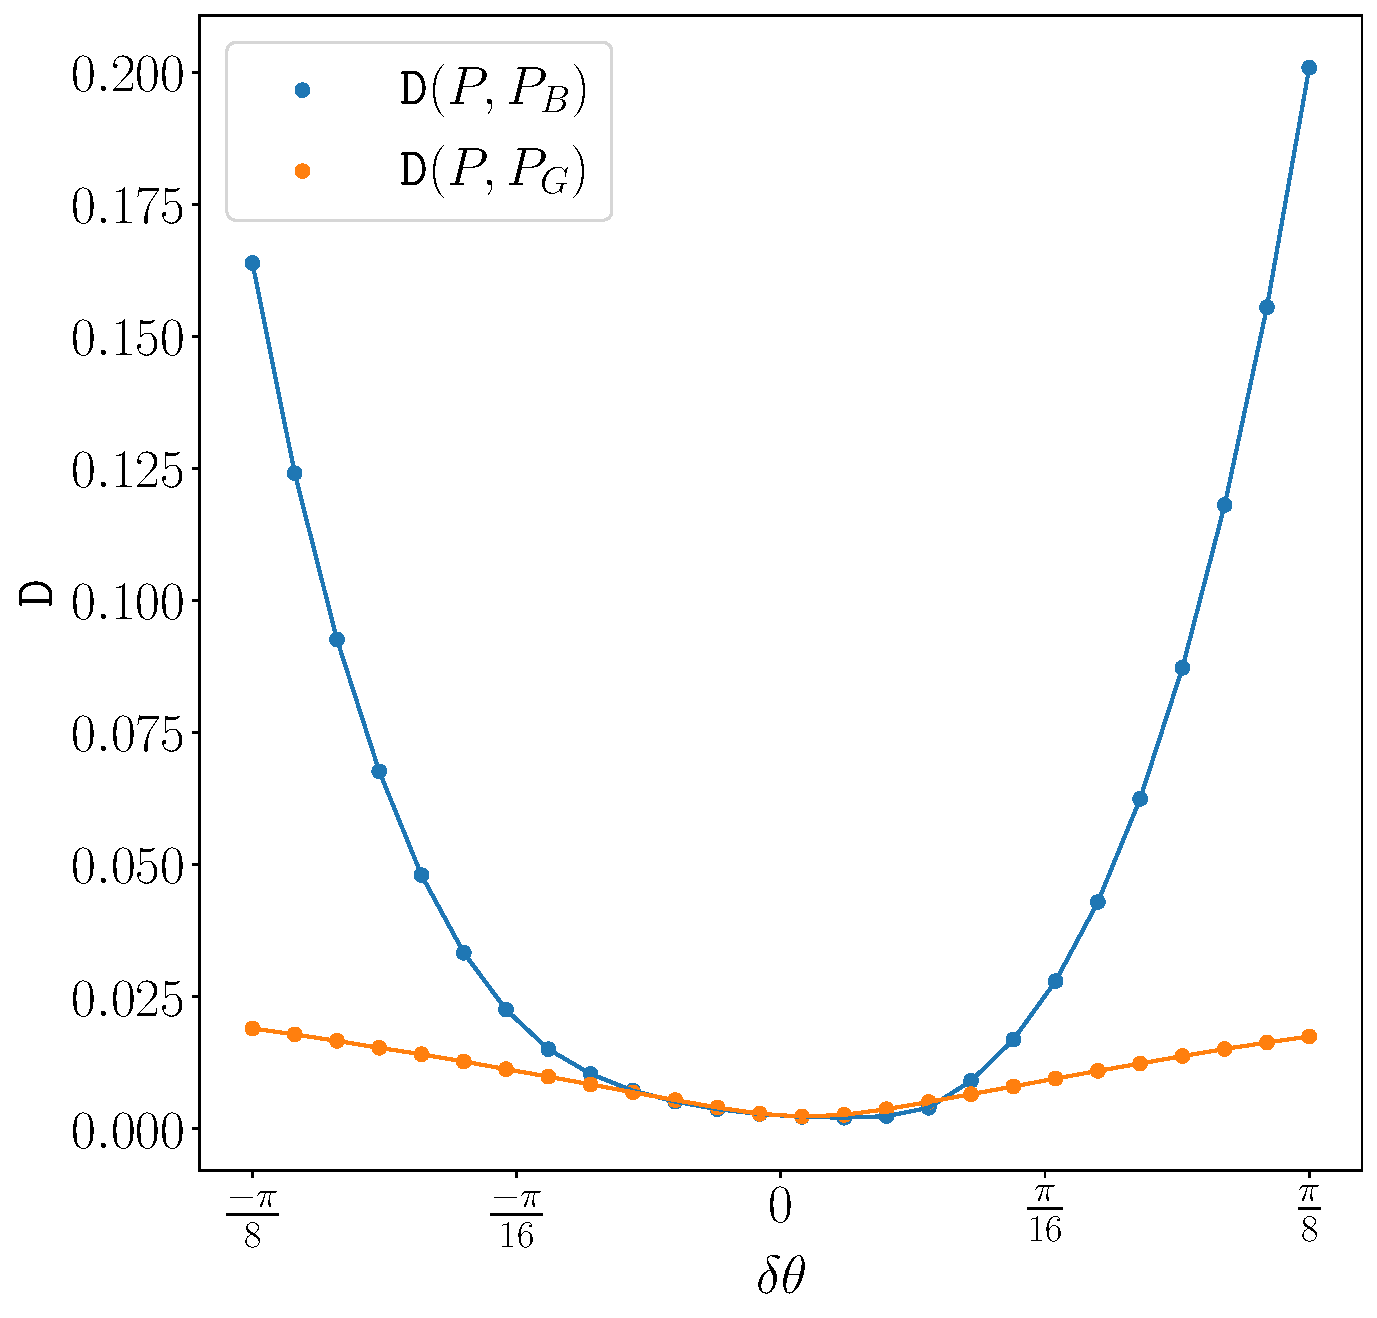
\includegraphics[width=\linewidth]{pics/appendix/theta.pdf}
    \caption{Distance between the exact statistical distribution and Gaussian (orange) and Skellam-based Gaussian (blue) approximations as a function of $\delta\theta$ with $\eta_1=\eta_2=1$. Note the significant difference (in first decimal places) between the curves, which means that $P_B$ becomes incorrect for higher asymmetry}
    \label{fig:PB_PG}
\end{figure}

\begin{figure}
    \centering
    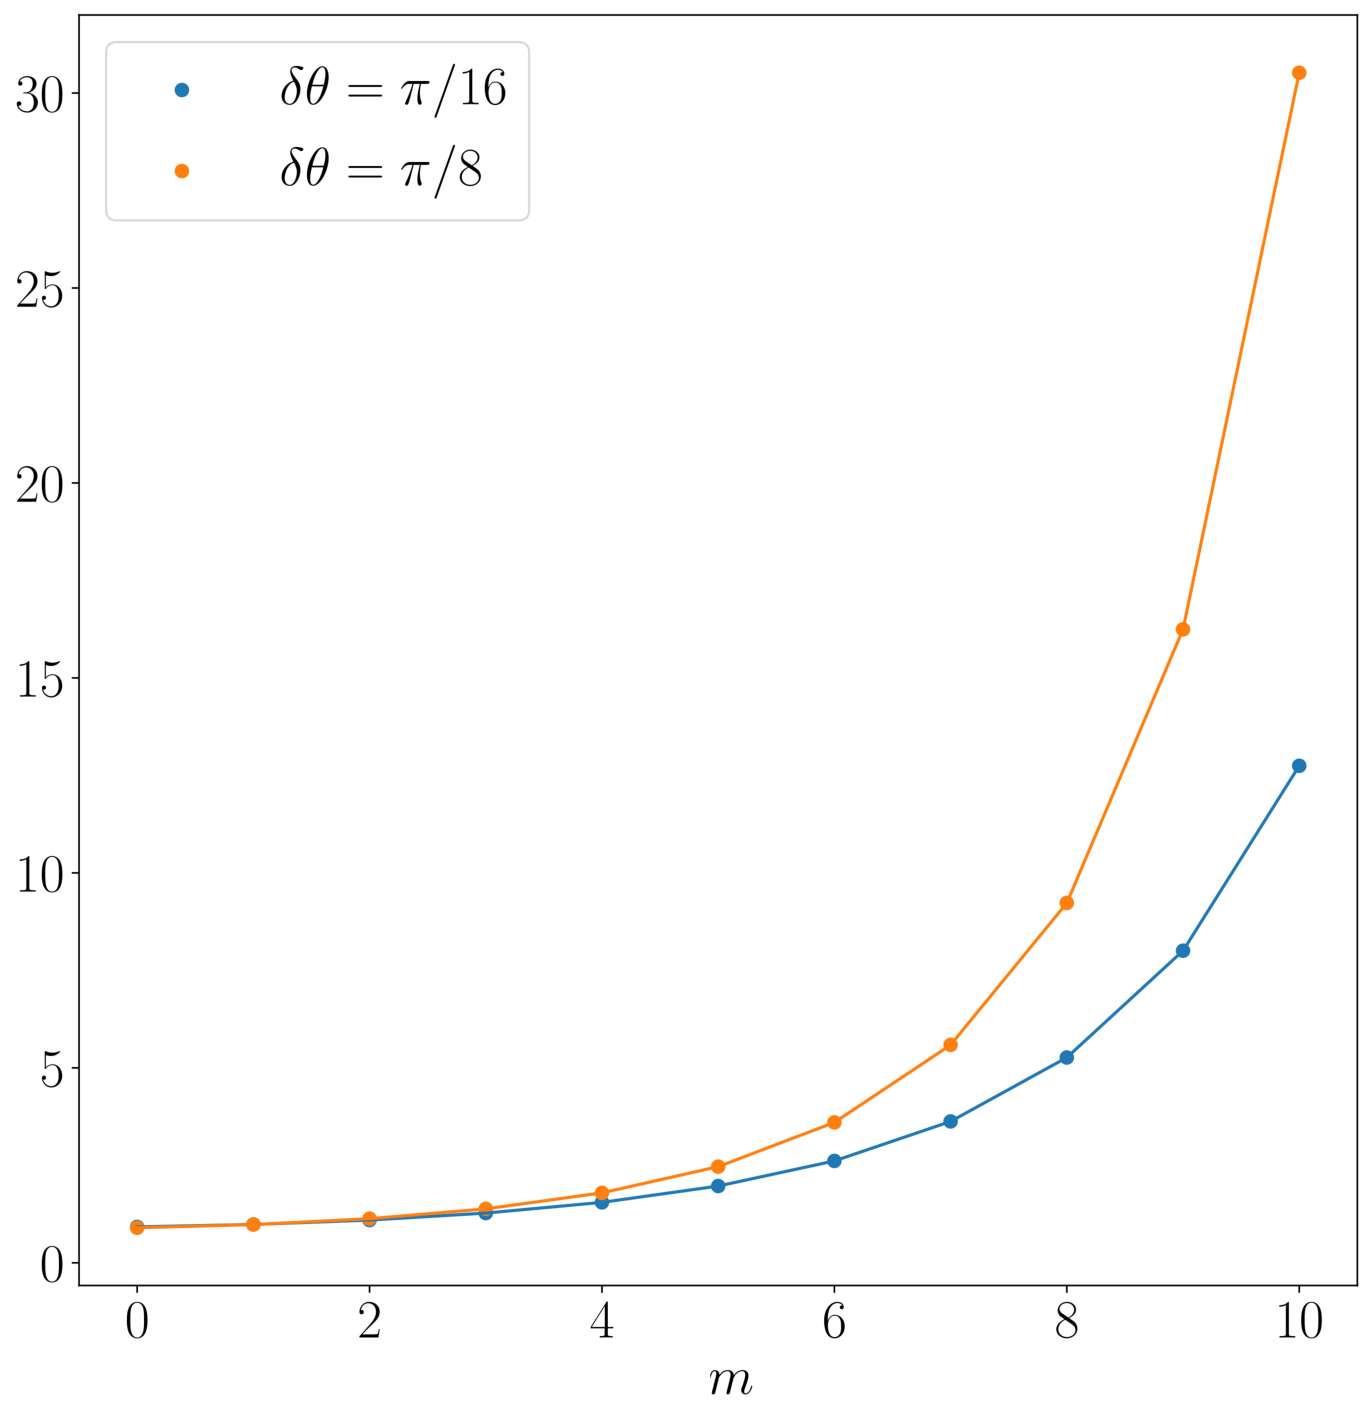
\includegraphics[width=0.75\linewidth]{pics/appendix/relation.pdf}
    \caption{Relation represented by Eq.~\eqref{eq:relation}, plotted against $\delta m$, with parameters $\eta_1=\eta_2=1, |\alpha|=0.1$ and $|\alpha_L|=5$, for various $\delta\theta$. Significant deviation from unity represents incorrectness of approximations Eq.~\eqref{eq:hole} and Eq.~\eqref{eq:hole2}.}
    \label{fig:relation}
\end{figure}